\chapter{Введение}

\section{Цель работы}

Цель работы – научиться исследовать электрические параметры фильтра <<Гранит>>.

Описание лабораторной установки:
\begin{enumerate}
	\item Осциллограф PV 6501A.
	\item Генератор тональных сигналов.
	\item Фильтр <<Гранит-8>>.
	\item Персональный компьютер;
\end{enumerate}


Фильтр предназначен для защиты от утечки информации за счёт акустоэлектрических преобразований и высокочастотного навязывания. Лабораторная установка собрана по следующей схеме:

\begin{figure}[H]
	\centering
	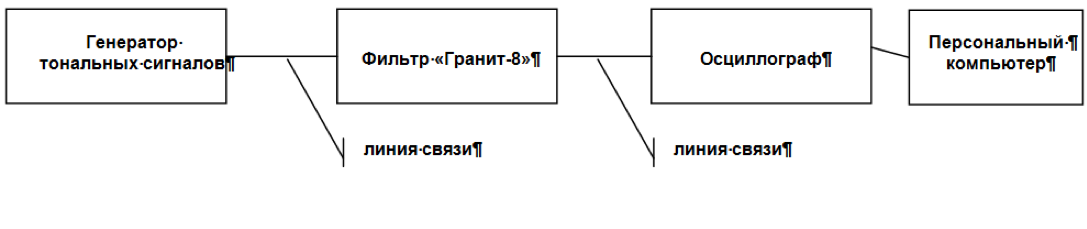
\includegraphics[width=\textwidth]{img/scheme.png}
	\caption{}
\end{figure}


\chapter{Ход работы}


\begin{figure}[H]
	\centering
	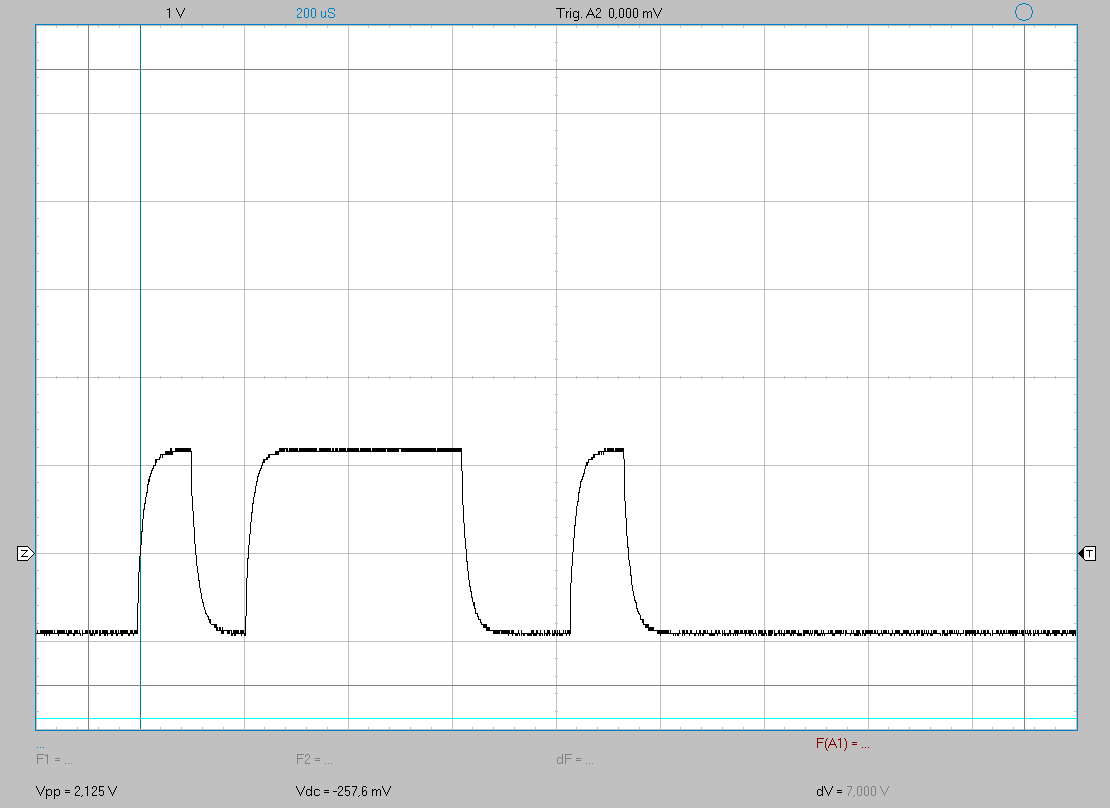
\includegraphics[width=\textwidth]{img/1.png}
	\caption{}
\end{figure}

\begin{figure}[H]
	\centering
	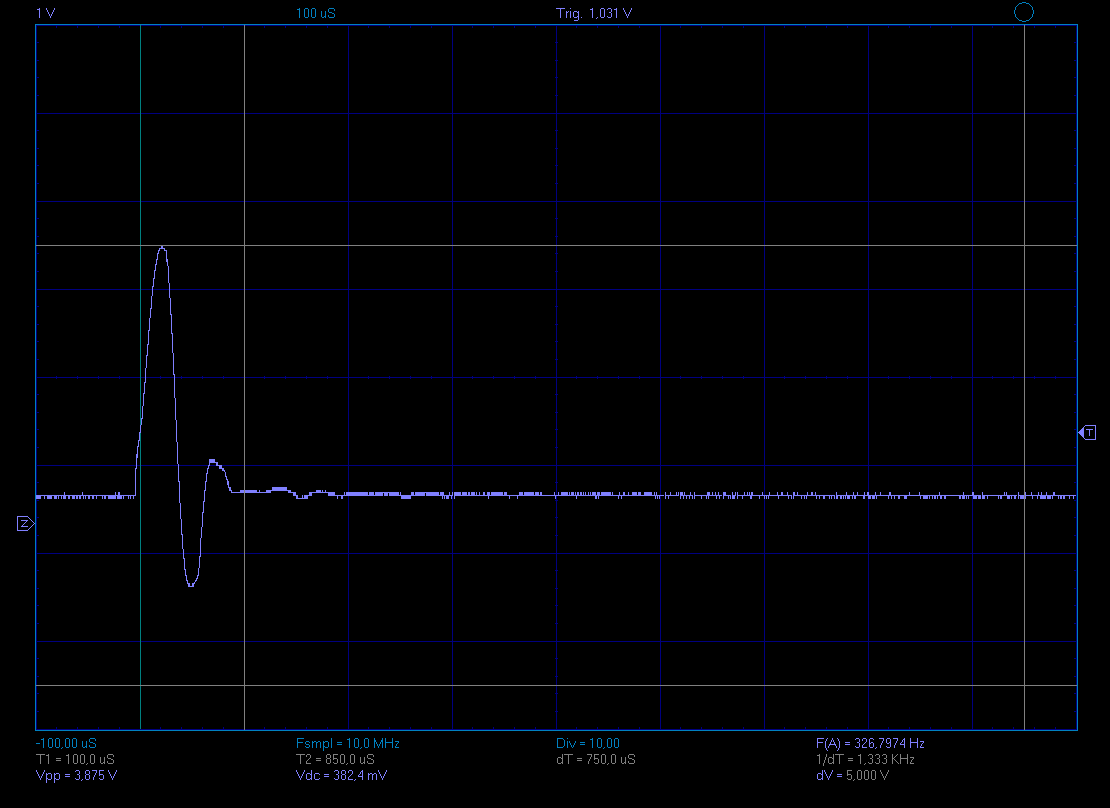
\includegraphics[width=\textwidth]{img/2.png}
	\caption{}
\end{figure}

\begin{table}[H]
	\centering
	\begin{tabular}{|l|l|l|}
		\hline
		f, Гц  & U, В & U, В \\ \hline
		100    & 4    & 3.25 \\ \hline
		250    & 4    & 3.20 \\ \hline
		500    & 4    & 3.15 \\ \hline
		1000   & 4    & 3.06 \\ \hline
		4000   & 4    & 3.03 \\ \hline
		10000  & 4    & 3.47 \\ \hline
		20000  & 4    & 5.13 \\ \hline
		30000  & 4    & 0.69 \\ \hline
		40000  & 4    & 0.70 \\ \hline
		50000  & 4    & 0.94 \\ \hline
		60000  & 4    & 1.06 \\ \hline
		70000  & 4    & 1.09 \\ \hline
		80000  & 4    & 1.10 \\ \hline
		90000  & 4    & 1.09 \\ \hline
		100000 & 4    & 1.06 \\ \hline
	\end{tabular}
	\caption{АЧХ фильтра <<Гранит-8>>}
\end{table}

\begin{tikzpicture}
\begin{axis}[
title={Зависимость коэффициента передачи от частоты.},
xlabel={Частота, Гц},
ylabel={U},
xmin=0, xmax=110000,
ymin=0, ymax=10,
legend pos=north west,
ymajorgrids=true,
grid style=dashed,
]

\addplot[
color=blue,
mark=square,
smooth
]
coordinates {
(100, 3.25)(250, 3.20)(500, 3.15)(1000, 3.06)(4000, 3.03)(10000, 3.47)(20000, 5.13)(30000, 0.69)(40000, 0.70)(50000, 0.94)(60000, 1.06)(70000, 1.09)(80000, 1.10)(90000, 1.09)(100000, 1.06)
};
\end{axis}
\end{tikzpicture}







